%%%%%%%%%%%%%%%%%%%%%%%%%%%%%%%%%%%%%%%%%%%%%%%%%%%%%%%%%%%%%%%%%%%%%%%%%%%
%% This file is part of the book
%%
%% Algorithmic Graph Theory
%% http://code.google.com/p/graph-theory-algorithms-book/
%%
%% Copyright (C) 2009, 2010, 2011 Minh Van Nguyen <nguyenminh2@gmail.com>
%% Copyright (C) 2010 Nathann Cohen <nathann.cohen@gmail.com>
%%
%% See the file COPYING for copying conditions.
%%%%%%%%%%%%%%%%%%%%%%%%%%%%%%%%%%%%%%%%%%%%%%%%%%%%%%%%%%%%%%%%%%%%%%%%%%%

\chapter{Random Graphs}
\label{chap:random_graphs}

A random\index{random graph} graph can be thought of as being a member
from a collection of graphs having some common properties. Recall that
Algorithm~\ref{alg:trees_forests:random_binary_tree} allows for
generating a random binary tree having at least one vertex. Fix a
positive integer $n$ and let $\cT$ be a collection of all binary trees
on $n$ vertices. It can be infeasible to generate all members of
$\cT$, so for most purposes we are only interested in randomly
generating a member of $\cT$. A binary tree of order $n$ generated in
this manner is said to be a random\index{random graph} graph. For
example, Algorithm~\ref{alg:random_graphs:random_simple_graph}
presents a procedure to construct a random graph that is simple and
undirected; the procedure is adapted from pages~4--7 of
Lau~\cite{Lau2007}.

\begin{itemize}
\item See Bollob{\'a}s~\cite{Bollobas2001}.

\item See Gerke~et~al.~\cite{GerkeEtAl2008} for a random planar graph
  process.

\item See Fusy~\cite{Fusy2009} for a linear algorithm on uniform
  random sampling of planar graphs.

\item See Broutin~\cite{Broutin2007} on random trees.
\end{itemize}

\begin{algorithm}[!htbp]
\index{algorithm!random}
\index{simple graph!random}
%%%%%%%%%%%%%%%%%%%%%%%%%%%%%%%%%%%%%%%%%%%%%%%%%%%%%%%%%%%%%%%%%%%%%%%%%%%
%% This file is part of the book
%%
%% Algorithmic Graph Theory
%% http://code.google.com/p/graph-theory-algorithms-book/
%%
%% Copyright (C) 2009, 2010, 2011 Minh Van Nguyen <nguyenminh2@gmail.com>
%%
%% See the file COPYING for copying conditions.
%%%%%%%%%%%%%%%%%%%%%%%%%%%%%%%%%%%%%%%%%%%%%%%%%%%%%%%%%%%%%%%%%%%%%%%%%%%

\DontPrintSemicolon
\SetAlgoNoLine
%%
%% data section
\SetKwData{MyFalse}{False}
\SetKwData{MyMax}{max}
\SetKwData{MyTrue}{True}
%%
%% input
\KwIn{Positive integers $n$ and $m$ specifying the order and size,
  respectively, of the output graph.}
%%
%% output
\KwOut{A random simple undirected graph with $n$ vertices and $m$
  edges. If $m$ exceeds the size of $K_n$, then $K_n$ is returned.}
\BlankLine
%%
%% algorithm body
\If{$n = 1$}{
  \Return $K_1$\;
}
$\MyMax \assign n(n - 1) / 2$\;
\If{$m > \MyMax$}{
  \Return $K_n$\;
}
$G \assign$ null graph\;
$A \assign n \times n$ adjacency matrix with entries $a_{ij}$\;
$a_{ij} \assign \MyFalse$ for $0 \leq i,j < n$\;
$i \assign 0$\;
\While{$i < m$}{
  $u \assign$ draw uniformly at random from $\{0, 1, \dots, n-1\}$\;
  $v \assign$ draw uniformly at random from $\{0, 1, \dots, n-1\}$\;
  \If{$u = v$}{
    continue with next iteration of loop\;
  }
  \If{$u > v$}{
    swap values of $u$ and $v$\;
  }
  \If{$a_{uv} = \MyFalse$}{
    add edge $uv$ to $G$\;
    $a_{uv} \assign \MyTrue$\;
    $i \assign i + 1$\;
  }
}
\Return $G$\;

\caption{Random simple undirected graph.}
\label{alg:random_graphs:random_simple_graph}
\end{algorithm}

\begin{algorithm}[!htbp]
\index{algorithm!random}
\index{simple graph!random}
%%%%%%%%%%%%%%%%%%%%%%%%%%%%%%%%%%%%%%%%%%%%%%%%%%%%%%%%%%%%%%%%%%%%%%%%%%%
%% This file is part of the book
%%
%% Algorithmic Graph Theory
%% http://code.google.com/p/graph-theory-algorithms-book/
%%
%% Copyright (C) 2009--2011 Minh Van Nguyen <nguyenminh2@gmail.com>
%%
%% See the file COPYING for copying conditions.
%%%%%%%%%%%%%%%%%%%%%%%%%%%%%%%%%%%%%%%%%%%%%%%%%%%%%%%%%%%%%%%%%%%%%%%%%%%

\DontPrintSemicolon
\SetAlgoNoLine
%%
%% input
\KwIn{Positive integer $n$ and a probability $0 < p < 1$.}
%%
%% output
\KwOut{A random graph from $G(n,p)$.}
\BlankLine
%%
%% algorithm body
$G \assign \overline{K_n}$\;
$V \assign \{0, 1, \dots, n - 1\}$\;
$E \assign$ $\{2$-combinations of $V\}$\;
\For{\rm each $e \in E$}{
  $r \assign$ draw uniformly at random from interval $(0,1)$\;
  \If{$r < p$}{
    add edge $e$ to $G$\;
  }
}
\Return $G$\;

\caption{Generate a random graph in $\cG(n,p)$.}
\label{alg:random_graphs:generate_random_Gnp}
\end{algorithm}


%% This section considers two closely related common models of random
%% graphs: the binomial model and the Erd\H{o}s-R\'enyi model. Both
%% models are considered to be processes for generating undirected simple
%% graphs satisfying certain parameters.


%%%%%%%%%%%%%%%%%%%%%%%%%%%%%%%%%%%%%%%%%%%%%%%%%%%%%%%%%%%%%%%%%%%%%%%%%%%

\section{Binomial random graph model}

Fix a positive integer $n$, a probability $p$, and a vertex set
$V = \{0, 1, \dots, n - 1\}$. The
\emph{binomial}\index{random graph!binomial}~(or
\emph{Bernoulli})\index{random graph!Bernoulli} random graph model,
denoted $\cG(n,p)$ and introduced by Gilbert~\cite{Gilbert1959}, is
formally a probability\index{probability!space} space over the set of
undirected simple graphs on $n$ vertices. If $G$ is any element of the
probability space $\cG(n,p)$ and $ij$ is any edge for distinct
$i,j \in V$, then $ij$ occurs as an edge of $G$ independently with
probability $p$. In symbols, for any distinct pair $i,j \in V$ we have
\[
\Pr[ij \in E(G)]
=
p
\]
where all such events are mutually independent. Equivalently the model
$\cG(n,p)$ considers the collection of all undirected simple graphs on
$n$ vertices, each such graph having at most $\binom{n}{2}$ edges, $m$
actual edges, and an associated probability
%%
\begin{equation}
\label{eqn:random_graphs:probability_of_chosen_graph_binomial_model}
p^m (1 - p)^{\binom{n}{2} - m}.
\end{equation}
%%
Notice the latter's resemblance to the
binomial\index{binomial!distribution} distribution. By
$G \in \cG(n,p)$ we mean that $G$ is a random graph of the space
$\cG(n,p)$ and having probability
distribution $\cG(n,p)$.

To generate a random graph in $\cG(n,p)$, start with $G$ being a graph
on $n$ vertices but no edges. Consider each of the $\binom{n}{2}$
possible edges in some order and add it independently to $G$ with
probability $p$. See
Algorithm~\ref{alg:random_graphs:generate_random_Gnp} for pseudocode
of the procedure. The runtime of
Algorithm~\ref{alg:random_graphs:generate_random_Gnp} depends on an
efficient algorithm for generating all $2$-combinations of a set of
$n$ objects. We could adapt
Algorithm~\ref{alg:tree_data_structures:generate_all_r_combinations}
to our needs or search for a more efficient algorithm; see
problem~\ref{chap:random_graphs}.\ref{prob:random_graphs:quadratic_generate_random_Gnp}
for discussion of an algorithm to generate a graph in $\cG(n,p)$ in
quadratic
time. Figure~\ref{fig:random_graphs:binomial_random_graph_25_nodes}
illustrates some graphs from $G(25,p)$ with $p = i/6$ for
$i = 0, 1, \dots, 5$.

The expected number of edges of any $G \in \cG(n,p)$ is
\[
\alpha
=
\E[|E|]
=
p \cdot \binom{n}{2}
=
\frac{p \cdot n!} {2! (n - 2)!}
\]
and the expected total degree is
\[
\beta
=
\E[\#\deg]
=
2p \cdot \binom{n}{2}
=
pn(n - 1).
\]
Then the expected degree of each edge is $p(n - 1)$. From
problem~\ref{chap:introduction}.\ref{prob:introduction:number_simple_graphs}
we know that the number of undirected simple graphs on $n$ vertices is
given by
\[
2^{n(n-1) / 2}
\]
where~\eqref{eqn:random_graphs:probability_of_chosen_graph_binomial_model}
is the probability of any of these graphs being the output of the
above procedure. Let $\kappa(n,m)$ be the number of graphs from
$\cG(n,p)$ that are connected and have size $m$, and by $\Pr[G_\kappa]$
is meant the probability that $G \in \cG(n,p)$ is connected. Apply
expression~\eqref{eqn:random_graphs:probability_of_chosen_graph_binomial_model}
to see that
\[
\Pr[G_\kappa]
=
\sum_{i=n-1}^{\binom{n}{2}}
\kappa(n,i) \cdot p^i (1 - p)^{\binom{n}{2} - i}
\]
where $n - 1$ is the least number of edges of any undirected connected
graph on $n$ vertices, i.e. the size of any spanning tree of a
connected graph in $\cG(n,p)$. Similarly define $\Pr[\kappa_{i,j}]$ to
be the probability that two distinct vertices $i,j$ of
$G \in \cG(n,p)$ are connected. Gilbert~\cite{Gilbert1959} showed that
as $n \to \infty$, the probabilities $\Pr[G_\kappa]$ and
$\Pr[\kappa_{i,j}]$ approach
\[
\Pr[G_\kappa] \to 1 - n(1 - p)^{n-1}
\]
and
\[
\Pr[\kappa_{i,j}] \to 1 - 2(1 - p)^{n-1}.
\]

\begin{figure}[!htbp]
\centering
\index{binomial!random graph}
%%%%%%%%%%%%%%%%%%%%%%%%%%%%%%%%%%%%%%%%%%%%%%%%%%%%%%%%%%%%%%%%%%%%%%%%%%%
%% This file is part of the book
%%
%% Algorithmic Graph Theory
%% http://code.google.com/p/graph-theory-algorithms-book/
%%
%% Copyright (C) 2009, 2010, 2011 Minh Van Nguyen <nguyenminh2@gmail.com>
%%
%% See the file COPYING for copying conditions.
%%%%%%%%%%%%%%%%%%%%%%%%%%%%%%%%%%%%%%%%%%%%%%%%%%%%%%%%%%%%%%%%%%%%%%%%%%%

\documentclass{article}

\usepackage{subfigure}
\usepackage{tikz}
\usetikzlibrary{external}
\tikzexternalize{binomial-random-graphs-25-nodes}

\begin{document}

\begin{figure}
\subfigure[$p = 0$;
  $\alpha = 0$, $|E| = 0$;
  $\beta = 0$, $\#\deg = 0$]{
\begin{tikzpicture}
[lineDecorate/.style={-,thick},%
  nodeDecorate/.style={shape=circle,inner sep=2pt,draw,thick},
  scale=3.4]
%% nodes or vertices
\foreach \nodename/\x/\y in {
  0/1.00000000000000/0.000000000000000,
  1/0.968583161128631/0.248689887164855,
  2/0.876306680043864/0.481753674101715,
  3/0.728968627421412/0.684547105928689,
  4/0.535826794978997/0.844327925502015,
  5/0.309016994374947/0.951056516295154,
  6/0.0627905195293135/0.998026728428272,
  7/-0.187381314585725/0.982287250728689,
  8/-0.425779291565073/0.904827052466019,
  9/-0.637423989748690/0.770513242775789,
  10/-0.809016994374947/0.587785252292473,
  11/-0.929776485888251/0.368124552684678,
  12/-0.992114701314478/0.125333233564305,
  13/-0.992114701314478/-0.125333233564304,
  14/-0.929776485888251/-0.368124552684678,
  15/-0.809016994374947/-0.587785252292473,
  16/-0.637423989748690/-0.770513242775789,
  17/-0.425779291565072/-0.904827052466020,
  18/-0.187381314585725/-0.982287250728689,
  19/0.0627905195293128/-0.998026728428272,
  20/0.309016994374947/-0.951056516295154,
  21/0.535826794978996/-0.844327925502016,
  22/0.728968627421411/-0.684547105928689,
  23/0.876306680043864/-0.481753674101715,
  24/0.968583161128631/-0.248689887164855}
{
  \node (\nodename) at (\x,\y) [nodeDecorate] {};
}
\end{tikzpicture}
}
%%
%%
\qquad
\subfigure[$p = 1/6$;
  $\alpha = 50$, $|E| = 44$;
  $\beta = 100$, $\#\deg = 88$]{
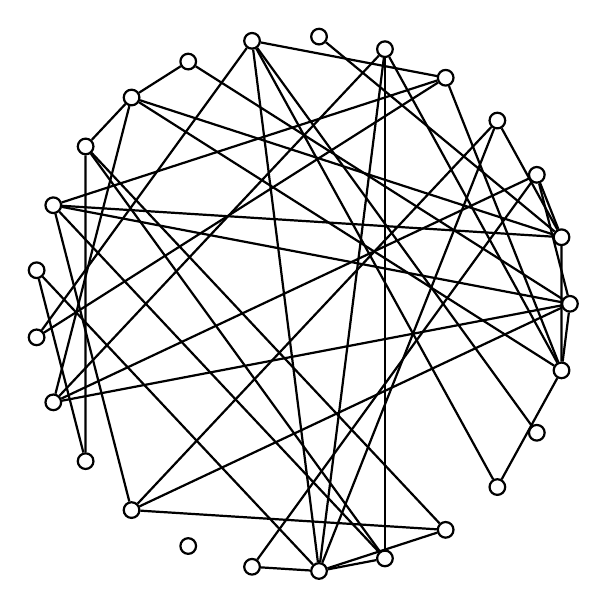
\begin{tikzpicture}
[lineDecorate/.style={-,thick},%
  nodeDecorate/.style={shape=circle,inner sep=2pt,draw,thick},
  scale=3.4]
%% nodes or vertices
\foreach \nodename/\x/\y in {
  0/1.00000000000000/0.000000000000000,
  1/0.968583161128631/0.248689887164855,
  2/0.876306680043864/0.481753674101715,
  3/0.728968627421412/0.684547105928689,
  4/0.535826794978997/0.844327925502015,
  5/0.309016994374947/0.951056516295154,
  6/0.0627905195293135/0.998026728428272,
  7/-0.187381314585725/0.982287250728689,
  8/-0.425779291565073/0.904827052466019,
  9/-0.637423989748690/0.770513242775789,
  10/-0.809016994374947/0.587785252292473,
  11/-0.929776485888251/0.368124552684678,
  12/-0.992114701314478/0.125333233564305,
  13/-0.992114701314478/-0.125333233564304,
  14/-0.929776485888251/-0.368124552684678,
  15/-0.809016994374947/-0.587785252292473,
  16/-0.637423989748690/-0.770513242775789,
  17/-0.425779291565072/-0.904827052466020,
  18/-0.187381314585725/-0.982287250728689,
  19/0.0627905195293128/-0.998026728428272,
  20/0.309016994374947/-0.951056516295154,
  21/0.535826794978996/-0.844327925502016,
  22/0.728968627421411/-0.684547105928689,
  23/0.876306680043864/-0.481753674101715,
  24/0.968583161128631/-0.248689887164855}
{
  \node (\nodename) at (\x,\y) [nodeDecorate] {};
}
%% edges or lines
\path
\foreach \startnode/\endnode in {
  0/2, 0/8, 0/11, 0/14, 0/16, 0/24, 1/2, 1/3, 1/6, 1/9, 1/11, 1/24,
  2/14, 2/18, 3/16, 3/19, 4/7, 4/11, 4/13, 4/24, 5/14, 5/19, 5/20, 5/24,
  7/13, 7/19, 7/22, 7/23, 8/9, 9/10, 9/14, 9/24, 10/15, 10/20, 10/21,
  11/16, 11/20, 12/15, 12/19, 16/21, 18/19, 19/20, 19/21, 22/24}
{
  (\startnode) edge[lineDecorate] node {} (\endnode)
};
\end{tikzpicture}
}
%%
%%
\subfigure[$p = 1/3$;
  $\alpha = 100$, $|E| = 108$;
  $\beta = 200$, $\#\deg = 212$]{
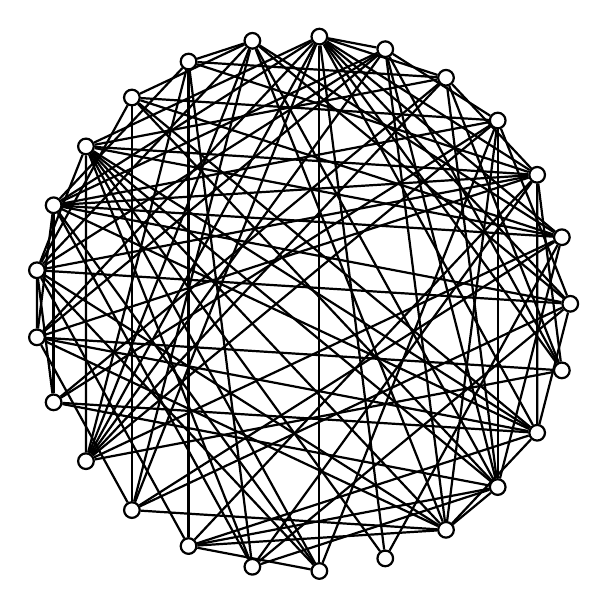
\begin{tikzpicture}
[lineDecorate/.style={-,thick},%
  nodeDecorate/.style={shape=circle,inner sep=2pt,draw,thick},
  scale=3.4]
%% nodes or vertices
\foreach \nodename/\x/\y in {
  0/1.00000000000000/0.000000000000000,
  1/0.968583161128631/0.248689887164855,
  2/0.876306680043864/0.481753674101715,
  3/0.728968627421412/0.684547105928689,
  4/0.535826794978997/0.844327925502015,
  5/0.309016994374947/0.951056516295154,
  6/0.0627905195293135/0.998026728428272,
  7/-0.187381314585725/0.982287250728689,
  8/-0.425779291565073/0.904827052466019,
  9/-0.637423989748690/0.770513242775789,
  10/-0.809016994374947/0.587785252292473,
  11/-0.929776485888251/0.368124552684678,
  12/-0.992114701314478/0.125333233564305,
  13/-0.992114701314478/-0.125333233564304,
  14/-0.929776485888251/-0.368124552684678,
  15/-0.809016994374947/-0.587785252292473,
  16/-0.637423989748690/-0.770513242775789,
  17/-0.425779291565072/-0.904827052466020,
  18/-0.187381314585725/-0.982287250728689,
  19/0.0627905195293128/-0.998026728428272,
  20/0.309016994374947/-0.951056516295154,
  21/0.535826794978996/-0.844327925502016,
  22/0.728968627421411/-0.684547105928689,
  23/0.876306680043864/-0.481753674101715,
  24/0.968583161128631/-0.248689887164855}
{
  \node (\nodename) at (\x,\y) [nodeDecorate] {};
}
%% edges or lines
\path
\foreach \startnode/\endnode in {
  0/3, 0/6, 0/7, 0/11, 0/12, 0/16, 0/18, 0/23, 1/6, 1/7, 1/9, 1/10,
  1/11, 1/15, 1/16, 1/20, 1/22, 2/4, 2/6, 2/8, 2/10, 2/11, 2/12, 2/13,
  2/17, 2/18, 2/23, 2/24, 3/5, 3/9, 3/11, 3/14, 3/15, 3/19, 3/21, 3/22,
  4/6, 4/8, 4/10, 4/14, 4/15, 4/22, 4/24, 5/6, 5/11, 5/12, 5/13, 5/15,
  5/21, 5/22, 5/24, 6/10, 6/11, 6/13, 6/15, 6/16, 6/19, 6/20, 6/23,
  6/24, 7/8, 7/9, 7/12, 7/15, 7/16, 7/21, 7/22, 8/11, 8/15, 8/17, 8/18,
  9/12, 9/16, 9/22, 9/23, 10/12, 10/15, 10/18, 10/19, 10/20, 10/21,
  10/22, 10/23, 11/13, 11/14, 11/18, 11/19, 11/23, 12/13, 12/14, 12/17,
  12/19, 12/21, 13/16, 13/21, 13/23, 13/24, 14/22, 14/23, 15/24, 16/21,
  17/19, 17/21, 17/22, 17/23, 18/22, 21/22, 21/23}
{
  (\startnode) edge[lineDecorate] node {} (\endnode)
};
\end{tikzpicture}
}
%%
%%
\qquad
\subfigure[$p = 1/2$;
  $\alpha = 150$, $|E| = 156$;
  $\beta = 300$, $\#\deg = 312$]{
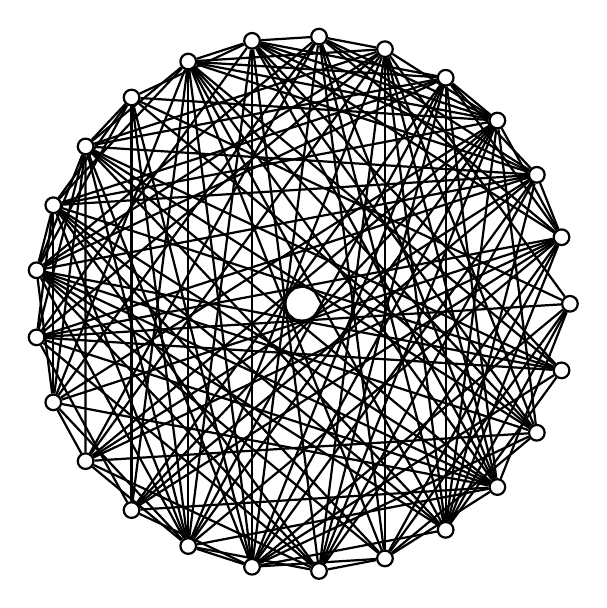
\begin{tikzpicture}
[lineDecorate/.style={-,thick},%
  nodeDecorate/.style={shape=circle,inner sep=2pt,draw,thick},
  scale=3.4]
%% nodes or vertices
\foreach \nodename/\x/\y in {
  0/1.00000000000000/0.000000000000000,
  1/0.968583161128631/0.248689887164855,
  2/0.876306680043864/0.481753674101715,
  3/0.728968627421412/0.684547105928689,
  4/0.535826794978997/0.844327925502015,
  5/0.309016994374947/0.951056516295154,
  6/0.0627905195293135/0.998026728428272,
  7/-0.187381314585725/0.982287250728689,
  8/-0.425779291565073/0.904827052466019,
  9/-0.637423989748690/0.770513242775789,
  10/-0.809016994374947/0.587785252292473,
  11/-0.929776485888251/0.368124552684678,
  12/-0.992114701314478/0.125333233564305,
  13/-0.992114701314478/-0.125333233564304,
  14/-0.929776485888251/-0.368124552684678,
  15/-0.809016994374947/-0.587785252292473,
  16/-0.637423989748690/-0.770513242775789,
  17/-0.425779291565072/-0.904827052466020,
  18/-0.187381314585725/-0.982287250728689,
  19/0.0627905195293128/-0.998026728428272,
  20/0.309016994374947/-0.951056516295154,
  21/0.535826794978996/-0.844327925502016,
  22/0.728968627421411/-0.684547105928689,
  23/0.876306680043864/-0.481753674101715,
  24/0.968583161128631/-0.248689887164855}
{
  \node (\nodename) at (\x,\y) [nodeDecorate] {};
}
%% edges or lines
\path
\foreach \startnode/\endnode in {
  0/5, 0/9, 0/13, 0/18, 0/20, 0/21, 0/22, 1/2, 1/3, 1/4, 1/6, 1/7, 1/13,
  1/14, 1/15, 1/16, 1/17, 1/19, 1/20, 1/21, 2/4, 2/6, 2/7, 2/8, 2/10,
  2/11, 2/12, 2/13, 2/15, 2/16, 2/18, 2/19, 2/21, 3/4, 3/5, 3/6, 3/7,
  3/8, 3/9, 3/11, 3/14, 3/15, 3/16, 3/17, 3/18, 3/19, 3/21, 3/23, 4/7,
  4/8, 4/10, 4/11, 4/12, 4/16, 4/17, 4/18, 4/19, 4/21, 4/22, 5/6, 5/8,
  5/10, 5/12, 5/13, 5/15, 5/17, 5/19, 5/20, 5/21, 5/22, 5/23, 6/7, 6/12,
  6/14, 6/15, 6/18, 6/20, 6/21, 6/22, 7/8, 7/9, 7/13, 7/17, 7/18, 7/19,
  7/22, 7/23, 7/24, 8/10, 8/11, 8/14, 8/16, 8/17, 8/18, 8/20, 8/21,
  8/22, 8/23, 8/24, 9/10, 9/11, 9/12, 9/16, 9/17, 9/18, 9/23, 10/12,
  10/13, 10/14, 10/15, 10/17, 10/18, 10/21, 10/22, 10/23, 10/24, 11/12,
  11/13, 11/14, 11/17, 11/19, 11/20, 11/21, 11/22, 11/24, 12/14, 12/17,
  12/19, 12/20, 12/21, 12/22, 12/23, 12/24, 13/16, 13/19, 13/22, 13/24,
  14/15, 14/17, 14/22, 15/17, 15/19, 15/23, 16/18, 16/22, 17/18, 17/19,
  17/22, 18/20, 18/21, 18/23, 18/24, 19/20, 20/22, 20/23, 21/24}
{
  (\startnode) edge[lineDecorate] node {} (\endnode)
};
\end{tikzpicture}
}
%%
%%
\subfigure[$p = 2/3$;
  $\alpha = 200$, $|E| = 185$;
  $\beta = 400$, $\#\deg = 370$]{
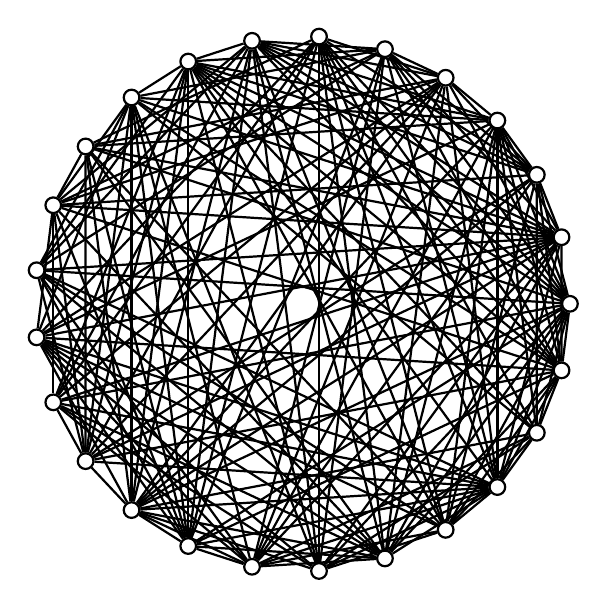
\begin{tikzpicture}
[lineDecorate/.style={-,thick},%
  nodeDecorate/.style={shape=circle,inner sep=2pt,draw,thick},
  scale=3.4]
%% nodes or vertices
\foreach \nodename/\x/\y in {
  0/1.00000000000000/0.000000000000000,
  1/0.968583161128631/0.248689887164855,
  2/0.876306680043864/0.481753674101715,
  3/0.728968627421412/0.684547105928689,
  4/0.535826794978997/0.844327925502015,
  5/0.309016994374947/0.951056516295154,
  6/0.0627905195293135/0.998026728428272,
  7/-0.187381314585725/0.982287250728689,
  8/-0.425779291565073/0.904827052466019,
  9/-0.637423989748690/0.770513242775789,
  10/-0.809016994374947/0.587785252292473,
  11/-0.929776485888251/0.368124552684678,
  12/-0.992114701314478/0.125333233564305,
  13/-0.992114701314478/-0.125333233564304,
  14/-0.929776485888251/-0.368124552684678,
  15/-0.809016994374947/-0.587785252292473,
  16/-0.637423989748690/-0.770513242775789,
  17/-0.425779291565072/-0.904827052466020,
  18/-0.187381314585725/-0.982287250728689,
  19/0.0627905195293128/-0.998026728428272,
  20/0.309016994374947/-0.951056516295154,
  21/0.535826794978996/-0.844327925502016,
  22/0.728968627421411/-0.684547105928689,
  23/0.876306680043864/-0.481753674101715,
  24/0.968583161128631/-0.248689887164855}
{
  \node (\nodename) at (\x,\y) [nodeDecorate] {};
}
%% edges or lines
\path
\foreach \startnode/\endnode in {
  0/2, 0/3, 0/4, 0/5, 0/6, 0/7, 0/8, 0/10, 0/12, 0/14, 0/16, 0/17, 0/19,
  0/20, 0/21, 0/22, 0/23, 0/24, 1/2, 1/3, 1/5, 1/7, 1/8, 1/9, 1/10,
  1/11, 1/12, 1/13, 1/14, 1/15, 1/16, 1/18, 1/19, 1/20, 1/22, 1/24, 2/3,
  2/4, 2/5, 2/6, 2/7, 2/8, 2/11, 2/15, 2/16, 2/18, 2/21, 2/23, 2/24,
  3/4, 3/7, 3/8, 3/9, 3/10, 3/13, 3/16, 3/18, 3/20, 3/21, 3/22, 3/23,
  3/24, 4/5, 4/6, 4/7, 4/10, 4/11, 4/13, 4/14, 4/15, 4/16, 4/18, 4/20,
  4/22, 5/7, 5/8, 5/9, 5/11, 5/12, 5/17, 5/18, 5/19, 5/22, 5/24, 6/10,
  6/13, 6/14, 6/15, 6/17, 6/19, 6/20, 6/21, 6/22, 6/23, 6/24, 7/8, 7/11,
  7/12, 7/14, 7/16, 7/17, 7/19, 7/20, 7/21, 7/24, 8/9, 8/12, 8/14, 8/15,
  8/16, 8/17, 8/19, 8/21, 8/22, 8/23, 8/24, 9/11, 9/12, 9/13, 9/15,
  9/16, 9/17, 9/18, 9/19, 9/23, 9/24, 10/11, 10/15, 10/16, 10/17, 10/20,
  10/21, 11/13, 11/14, 11/15, 11/17, 11/20, 11/24, 12/15, 12/17, 12/18,
  12/20, 12/21, 12/22, 13/16, 13/17, 13/18, 13/19, 13/20, 13/21, 13/22,
  13/24, 14/15, 14/18, 14/19, 14/20, 14/22, 15/16, 15/22, 15/24, 16/17,
  16/18, 16/19, 16/20, 16/22, 16/23, 17/18, 17/20, 17/22, 17/24, 18/20,
  18/21, 18/22, 18/23, 19/21, 19/22, 19/23, 20/22, 20/24, 21/22, 21/23,
  21/24, 22/23, 22/24, 23/24}
{
  (\startnode) edge[lineDecorate] node {} (\endnode)
};
\end{tikzpicture}
}
%%
%%
\qquad
\subfigure[$p = 5/6$;
  $\alpha = 250$, $|E| = 255$;
  $\beta = 500$, $\#\deg = 510$]{
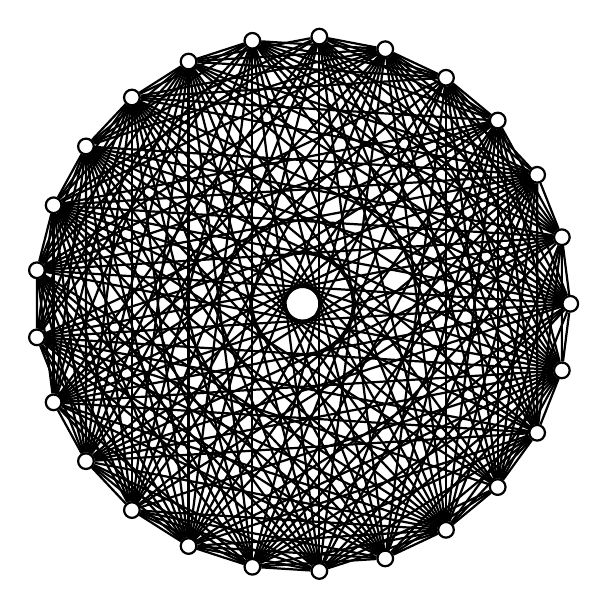
\begin{tikzpicture}
[lineDecorate/.style={-,thick},%
  nodeDecorate/.style={shape=circle,inner sep=2pt,draw,thick},
  scale=3.4]
%% nodes or vertices
\foreach \nodename/\x/\y in {
  0/1.00000000000000/0.000000000000000,
  1/0.968583161128631/0.248689887164855,
  2/0.876306680043864/0.481753674101715,
  3/0.728968627421412/0.684547105928689,
  4/0.535826794978997/0.844327925502015,
  5/0.309016994374947/0.951056516295154,
  6/0.0627905195293135/0.998026728428272,
  7/-0.187381314585725/0.982287250728689,
  8/-0.425779291565073/0.904827052466019,
  9/-0.637423989748690/0.770513242775789,
  10/-0.809016994374947/0.587785252292473,
  11/-0.929776485888251/0.368124552684678,
  12/-0.992114701314478/0.125333233564305,
  13/-0.992114701314478/-0.125333233564304,
  14/-0.929776485888251/-0.368124552684678,
  15/-0.809016994374947/-0.587785252292473,
  16/-0.637423989748690/-0.770513242775789,
  17/-0.425779291565072/-0.904827052466020,
  18/-0.187381314585725/-0.982287250728689,
  19/0.0627905195293128/-0.998026728428272,
  20/0.309016994374947/-0.951056516295154,
  21/0.535826794978996/-0.844327925502016,
  22/0.728968627421411/-0.684547105928689,
  23/0.876306680043864/-0.481753674101715,
  24/0.968583161128631/-0.248689887164855}
{
  \node (\nodename) at (\x,\y) [nodeDecorate] {};
}
%% edges or lines
\path
\foreach \startnode/\endnode in {
  0/1, 0/3, 0/4, 0/5, 0/6, 0/7, 0/8, 0/9, 0/10, 0/11, 0/12, 0/13, 0/14,
  0/15, 0/17, 0/18, 0/19, 0/22, 0/24, 1/2, 1/3, 1/4, 1/5, 1/6, 1/7, 1/8,
  1/10, 1/11, 1/12, 1/13, 1/14, 1/15, 1/16, 1/18, 1/21, 1/22, 1/23,
  1/24, 2/4, 2/5, 2/7, 2/8, 2/9, 2/10, 2/11, 2/12, 2/13, 2/14, 2/15,
  2/16, 2/17, 2/18, 2/19, 2/20, 2/21, 2/22, 2/23, 3/4, 3/5, 3/6, 3/7,
  3/9, 3/11, 3/12, 3/13, 3/14, 3/15, 3/17, 3/18, 3/19, 3/20, 3/21, 3/22,
  3/23, 3/24, 4/5, 4/6, 4/7, 4/8, 4/9, 4/12, 4/14, 4/16, 4/17, 4/18,
  4/20, 4/21, 4/22, 4/23, 4/24, 5/6, 5/7, 5/8, 5/9, 5/10, 5/11, 5/12,
  5/14, 5/15, 5/16, 5/17, 5/18, 5/19, 5/21, 5/22, 5/23, 5/24, 6/8, 6/10,
  6/11, 6/14, 6/15, 6/16, 6/17, 6/19, 6/20, 6/21, 6/22, 6/23, 6/24, 7/8,
  7/9, 7/10, 7/12, 7/13, 7/15, 7/16, 7/17, 7/18, 7/19, 7/20, 7/21, 7/23,
  7/24, 8/9, 8/10, 8/11, 8/12, 8/13, 8/14, 8/15, 8/16, 8/17, 8/18, 8/19,
  8/20, 8/21, 8/22, 8/24, 9/10, 9/11, 9/12, 9/13, 9/14, 9/15, 9/16,
  9/17, 9/18, 9/19, 9/20, 9/21, 9/22, 9/23, 9/24, 10/11, 10/12, 10/13,
  10/14, 10/15, 10/16, 10/17, 10/18, 10/19, 10/20, 10/21, 10/22, 10/23,
  10/24, 11/12, 11/13, 11/14, 11/15, 11/16, 11/17, 11/18, 11/19, 11/20,
  11/21, 11/22, 11/23, 11/24, 12/13, 12/14, 12/15, 12/16, 12/17, 12/18,
  12/19, 12/20, 12/21, 12/24, 13/15, 13/16, 13/17, 13/19, 13/20, 13/21,
  13/22, 13/23, 13/24, 14/15, 14/17, 14/18, 14/20, 14/21, 14/23, 14/24,
  15/16, 15/17, 15/18, 15/19, 15/21, 15/23, 15/24, 16/17, 16/18, 16/19,
  16/20, 16/21, 16/24, 17/18, 17/19, 17/20, 17/21, 17/23, 17/24, 18/19,
  18/20, 18/21, 18/23, 18/24, 19/21, 19/22, 19/23, 19/24, 20/21, 20/22,
  20/23, 20/24, 21/22, 21/23, 21/24, 22/23, 22/24, 23/24}
{
  (\startnode) edge[lineDecorate] node {} (\endnode)
};
\end{tikzpicture}
}
\end{figure}

\end{document}

\caption{Binomial random graphs $G(25,p)$ for various values of $p$.}
\label{fig:random_graphs:binomial_random_graph_25_nodes}
\end{figure}


%%%%%%%%%%%%%%%%%%%%%%%%%%%%%%%%%%%%%%%%%%%%%%%%%%%%%%%%%%%%%%%%%%%%%%%%%%%

\subsubsection{Efficient generation of sparse $G \in \cG(n,p)$}

The techniques discussed so
far~(Algorithms~\ref{alg:random_graphs:generate_random_Gnp}
and~\ref{alg:random_graphs:quadratic_generate_random_Gnp}) for
generating a random graph from $\cG(n,p)$ can be unsuitable when the
number of vertices $n$ is in the hundreds of thousands or millions. In
many applications of $\cG(n,p)$ we are only interested in
sparse\index{sparse graph} random graphs. A linear time algorithm to
generate a random sparse graph from $\cG(n,p)$ is presented in
Batagelj\index{Batagelj, Vladimir} and
Brandes\index{Brandes, Ulrik}~\cite{BatageljBrandes2005}.

The Batagelj-Brandes\index{Batagelj-Brandes algorithm} algorithm for
generating a random sparse graph $G \in \cG(n,p)$ uses what is known as
a geometric method to skip over certain edges. Fix a probability
$0 < p < 1$ that an edge will be in the resulting random sparse graph
$G$. If $e$ is an edge of $G$, we can consider the events leading up
to the choice of $e$ as
\[
e_1, e_2, \dots, e_k
\]
where in the $i$-th trial the event $e_i$ is a failure, for
$1 \leq i < k$, but the event $e_k$ is the first success after
$k - 1$ successive failures. In probabilistic terms, we perform a
series of independent trials each having success probability $p$ and
stop when the first success occurs. Letting $X$ be the number of
trials required until the first success occurs, then $X$ is a
geometric random variable with parameter $p$ and probability mass
function
%%
\begin{equation}
\label{eqn:random_graphs:probability_mass_function_geometric_distribution}
\Pr[X = k]
=
p (1 - p)^{k - 1}
\end{equation}
%%
for integers $k \geq 1$, where
\[
\sum_{k=1}^\infty p (1 - p)^{k - 1}
=
1.
\]
In other words, waiting times are
geometrically\index{distribution!geometric} distributed.

Suppose we want to generate a random
number\index{pseudorandom number} from a
geometric\index{distribution!geometric} distribution, i.e. we want to
simulate $X$ such that
\[
\Pr[X = k]
=
p (1 - p)^{k-1},
\qquad
k = 1, 2, 3, \dots
\]
Note that
\[
\sum_{k=1}^{\ell} \Pr[X=k]
=
1 - \Pr[X > \ell - 1]
=
1 - (1 - p)^{\ell - 1}.
\]
In other words, we can simulate a
geometric\index{random variable!geometric} random variable by
generating $r$ uniformly at random from the interval $(0,1)$ and set
$X$ to that value of $k$ for which
\[
1 - (1 - p)^{k-1} < r < 1 - (1 - p)^k
\]
or equivalently for which
\[
(1 - p)^k < 1 - r < (1 - p)^{k-1}
\]
where $1 - r$ and $r$ are both uniformly\index{distribution!uniform}
distributed. Thus we can define $X$ by
%%
\begin{align*}
X
&=
\min\{k \mid (1 - p)^k < 1 - r\} \\[4pt]
&=
\min\left\{
  k \;\left|\; k > \frac{\ln(1 - r)} {\ln(1 - p)} \right.
\right\} \\[4pt]
&=
1 + \left\lfloor \frac{\ln(1 - r)} {\ln(1 - p)} \right\rfloor.
\end{align*}
%%
That is, we can choose $k$ to be
\[
k
=
1 + \left\lfloor \frac{\ln(1 - r)} {\ln(1 - p)} \right\rfloor
\]
which is used as a basis of
Algorithm~\ref{alg:random_graphs:linear_generate_random_sparse_Gnp}. In
the latter algorithm, note that the vertex set is
$V = \{0, 1, \dots, n-1\}$ and candidate edges are generated in
lexicographic order. The Batagelj-Brandes
Algorithm~\ref{alg:random_graphs:linear_generate_random_sparse_Gnp}
has worst-case runtime $O(n + m)$, where $n$ and $m$ are the order and
size, respectively, of the resulting graph.

\begin{algorithm}[!htbp]
\index{algorithm!random}
\index{Batagelj-Brandes algorithm}
\index{complete graph}
\index{simple graph!random}
%%%%%%%%%%%%%%%%%%%%%%%%%%%%%%%%%%%%%%%%%%%%%%%%%%%%%%%%%%%%%%%%%%%%%%%%%%%
%% This file is part of the book
%%
%% Algorithmic Graph Theory
%% http://code.google.com/p/graph-theory-algorithms-book/
%%
%% Copyright (C) 2009, 2010, 2011 Minh Van Nguyen <nguyenminh2@gmail.com>
%%
%% See the file COPYING for copying conditions.
%%%%%%%%%%%%%%%%%%%%%%%%%%%%%%%%%%%%%%%%%%%%%%%%%%%%%%%%%%%%%%%%%%%%%%%%%%%

\DontPrintSemicolon
\SetAlgoNoLine
%%
%% data section
\SetKwInOut{Input}{Input}
\SetKwInOut{Output}{Output}
%%
%% input/output
\Input{Positive integer $n$ and a probability $0 < p < 1$.}
\Output{A random sparse graph from $G(n,p)$.}
\BlankLine
%%
%% algorithm body
$G \assign \overline{K_n}$\;
$u \assign 1$\;
$v \assign -1$\;
\While{$u < n$}{
  $r \assign$ draw uniformly at random from interval $(0,1)$\;
  $v \assign v + 1 + \lfloor \ln(1 - r) / \ln(1 - p) \rfloor$\;
  \While{\rm $v \geq u$ and $u < n$}{
    $v \assign v - u$\;
    $u \assign u + 1$\;
  }
  \If{$u < n$}{
    add edge $uv$ to $G$\;
  }
}
\Return $G$\;

\caption{Linear generation of a random sparse graph in $\cG(n,p)$.}
\label{alg:random_graphs:linear_generate_random_sparse_Gnp}
\end{algorithm}


%%%%%%%%%%%%%%%%%%%%%%%%%%%%%%%%%%%%%%%%%%%%%%%%%%%%%%%%%%%%%%%%%%%%%%%%%%%

\section{Erd\H{o}s-R\'enyi model}
\label{sec:random_graphs:Erdos_Renyi_model}

Let $N$ be a fixed nonnegative integer. The
\emph{Erd\H{o}s-R\'enyi}~\cite{ErdosRenyi1959,ErdosRenyi1960}
(or\index{random graph!Erd\H{o}s-R\'enyi}
\emph{uniform})\index{random graph!uniform} random graph model,
denoted $\cG(n,N)$, is a probability space over the set of undirected
simple graphs on $n$ vertices and exactly $N$ edges. Hence $\cG(n,N)$
can be considered as a collection of $\binom{\binom{n}{2}} {N}$
undirected simple graphs on exactly $N$ edges, each such graph being
selected with equal probability. A note of caution is in order
here. Numerous papers on random graphs refer to $\cG(n,p)$ as the
Erd\H{o}s-R\'enyi random graph model, where in fact this binomial
random graph model should be called the Gilbert model in honor of
E.~N.~Gilbert\index{Gilbert, E.~N.} who introduced~\cite{Gilbert1959}
it in~1959. Whenever a paper makes a reference to the
Erd\H{o}s-R\'enyi model, one should question whether the paper is
referring to $\cG(n,p)$ or $\cG(n,N)$.

To generate a graph in $\cG(n,N)$, start with $G$ being a graph on $n$
vertices but no edges. Then choose $N$ of the possible $\binom{n}{2}$
edges independently and uniformly at random and let the chosen edges
be the edge set of $G$. Each graph $G \in \cG(n,N)$ is associated with a
probability
\[
1 \left/ \binom{\binom{n}{2}} {N} \right.
\]
of being the graph resulting from the above procedure. Furthermore
each of the $\binom{n}{2}$ edges has a probability
\[
1 \left/ \binom{n}{2} \right.
\]
of being chosen.
Algorithm~\ref{alg:random_graphs:linear_generate_random_GnN} presents
a straightforward translation of the above procedure into pseudocode.

\begin{algorithm}[!htbp]
\index{algorithm!random}
\index{simple graph!random}
%%%%%%%%%%%%%%%%%%%%%%%%%%%%%%%%%%%%%%%%%%%%%%%%%%%%%%%%%%%%%%%%%%%%%%%%%%%
%% This file is part of the book
%%
%% Algorithmic Graph Theory
%% http://code.google.com/p/graph-theory-algorithms-book/
%%
%% Copyright (C) 2009, 2010, 2011 Minh Van Nguyen <nguyenminh2@gmail.com>
%%
%% See the file COPYING for copying conditions.
%%%%%%%%%%%%%%%%%%%%%%%%%%%%%%%%%%%%%%%%%%%%%%%%%%%%%%%%%%%%%%%%%%%%%%%%%%%

\DontPrintSemicolon
\SetAlgoNoLine
%%
%% data section
\SetKwInOut{Input}{Input}
\SetKwInOut{Output}{Output}
%%
%% input/output
\Input{Positive integer $n$ and integer $N$ with $0 \leq N \leq \binom{n}{2}$.}
\Output{A random graph from $G(n,N)$.}
\BlankLine
%%
%% algorithm body
$G \assign \overline{K_n}$\;
$E \assign \left\{e_0, e_1, \dots, e_{\binom{n}{2} - 1}\right\}$\;
\For{$i \assign 0, 1, \dots, N - 1$}{
  $r \assign$ draw uniformly at random from $\left\{0, 1, \dots, \binom{n}{2} - 1\right\}$\;
  \While{\rm $e_r$ is an edge of $G$}{
    $r \assign$ draw uniformly at random from $\left\{0, 1, \dots, \binom{n}{2} - 1\right\}$\;
  }
  add edge $e_r$ to $G$\;
}
\Return $G$\;

\caption{Generation of random graph in $\cG(n,N)$.}
\label{alg:random_graphs:linear_generate_random_GnN}
\end{algorithm}

The runtime of
Algorithm~\ref{alg:random_graphs:linear_generate_random_GnN} is
probabilistic and can be analyzed via the
geometric\index{distribution!geometric} distribution. If $i$ is the
number of edges chosen so far, then the probability of choosing a new
edge in the next step is
\[
\frac{\binom{n}{2} - i} {\binom{n}{2}}.
\]
We repeatedly choose an edge uniformly at random from the collection
of all possible edges, until we come across the first edge that is not
already in the graph. The number of trials required until the first
new edge is chosen can be modeled using the geometric distribution
with probability mass
function~\eqref{eqn:random_graphs:probability_mass_function_geometric_distribution}.
Given a geometric random variable $X$, we have the expectation
\[
\E[X]
=
\sum_{n=1}^\infty n \cdot p(1 - p)^{n-1}
=
\frac{1}{p}.
\]
Therefore the expected number of trials until a new edge be chosen is
\[
\frac{\binom{n}{2}} {\binom{n}{2} - i}
\]
from which the expected total runtime is
%%
\begin{align*}
\label{eqn:random_graphs:Erdos_Renyi_expected_total_runtime_sum}
\sum_{i=1}^N \frac{\binom{n}{2}} {\binom{n}{2} - i}
&\approx
\int_0^N \frac{\binom{n}{2}} {\binom{n}{2} - x} \; dx \\[4pt]
&=
\binom{n}{2} \cdot \ln \frac{\binom{n}{2}} {\binom{n}{2} - N}.
\end{align*}
%%
The denominator in the latter fraction becomes zero when
$\binom{n}{2} = N$, which can be prevented by adding one to the
denominator. Then we have the expected total runtime
\[
\sum_{i=1}^N \frac{\binom{n}{2}} {\binom{n}{2} - i}
\in
\Theta
\left(
  \binom{n}{2} \cdot \ln \frac{\binom{n}{2}} {\binom{n}{2} - N + 1}
\right)
\]
which is $O(N)$ when $N \leq \binom{n}{2} / 2$, and $O(N \cdot \ln N)$
when $N = \binom{n}{2}$. In other words,
Algorithm~\ref{alg:random_graphs:linear_generate_random_GnN} has
expected linear runtime when the number $N$ of required edges
satisfies $N \leq \binom{n}{2} / 2$. But for $N > \binom{n}{2} / 2$,
we obtain expected linear runtime by generating the
complete\index{complete graph} graph $K_n$ and randomly delete
$\binom{n}{2} - N$ edges from the latter graph. Our discussion is
summarized in
Algorithm~\ref{alg:random_graphs:expected_linear_generate_random_GnN}.

\begin{algorithm}[!htbp]
\index{algorithm!random}
\index{simple graph!random}
%%%%%%%%%%%%%%%%%%%%%%%%%%%%%%%%%%%%%%%%%%%%%%%%%%%%%%%%%%%%%%%%%%%%%%%%%%%
%% This file is part of the book
%%
%% Algorithmic Graph Theory
%% http://code.google.com/p/graph-theory-algorithms-book/
%%
%% Copyright (C) 2009, 2010, 2011 Minh Van Nguyen <nguyenminh2@gmail.com>
%%
%% See the file COPYING for copying conditions.
%%%%%%%%%%%%%%%%%%%%%%%%%%%%%%%%%%%%%%%%%%%%%%%%%%%%%%%%%%%%%%%%%%%%%%%%%%%

\DontPrintSemicolon
\SetAlgoNoLine
%%
%% input
\KwIn{Positive integer $n$ and integer $N$ with $0 \leq N \leq \binom{n}{2}$.}
%%
%% output
\KwOut{A random graph from $G(n,N)$.}
\BlankLine
%%
%% algorithm body
\If{$N \leq \binom{n}{2} / 2$}{
  \Return result of Algorithm~\ref{alg:random_graphs:linear_generate_random_GnN}\;
}
$G \assign K_n$\;
\For{$i \assign 1, 2, \dots, \binom{n}{2} - N$}{
  $e \assign$ draw uniformly at random from $E(G)$\;
  remove edge $e$ from $G$\;
}
\Return $G$\;

\caption{Generation of random graph in $\cG(n,N)$ in expected linear time.}
\label{alg:random_graphs:expected_linear_generate_random_GnN}
\end{algorithm}

\begin{algorithm}[!htbp]
\index{algorithm!random}
\index{oriented graph}
\index{oriented graph!random}
%%%%%%%%%%%%%%%%%%%%%%%%%%%%%%%%%%%%%%%%%%%%%%%%%%%%%%%%%%%%%%%%%%%%%%%%%%%
%% This file is part of the book
%%
%% Algorithmic Graph Theory
%% http://code.google.com/p/graph-theory-algorithms-book/
%%
%% Copyright (C) 2009, 2010, 2011 Minh Van Nguyen <nguyenminh2@gmail.com>
%%
%% See the file COPYING for copying conditions.
%%%%%%%%%%%%%%%%%%%%%%%%%%%%%%%%%%%%%%%%%%%%%%%%%%%%%%%%%%%%%%%%%%%%%%%%%%%

\DontPrintSemicolon
\SetAlgoNoLine
%%
%% data section
\SetKwInOut{Input}{Input}
\SetKwInOut{Output}{Output}
\SetKwData{MyCutOff}{cutoff}
%%
%% input/output
\Input{Positive integer $n$ and probability $0 < p < 1$.}
\Output{A random oriented graph on $n$ vertices.}
\BlankLine
%%
%% algorithm body
$G \assign$ random graph in $G(n,p)$ as per Algorithm~\ref{alg:random_graphs:linear_generate_random_sparse_Gnp}\;
$E \assign$ edge set of $G$\;
$G \assign$ directed version of $G$\;
$\MyCutOff \assign$ draw uniformly at random from $[0,1)$\;
\For{\rm each edge $uv \in E$}{
  $r \assign$ draw uniformly at random from $[0,1)$\;
  \eIf{$r < \MyCutOff$}{
    remove $uv$ from $G$\;
  }{
    remove $vu$ from $G$\;
  }
}
\Return $G$\;

\caption{Random oriented graph via $\cG(n,p)$.}
\label{alg:random_graphs:random_oriented_graph_Gnp}
\end{algorithm}

\begin{example}
\label{eg:random_graphs:random_oriented_graph}
Consider a digraph $D = (V,E)$ without self-loops or multiple
edges. Then $D$ is said to be \emph{oriented}\index{oriented graph} if
for any distinct pair $u,v \in V$ at most one of $uv, vu$ is an edge
of $D$. Provide specific examples of oriented graphs.
\end{example}

\begin{proof}[Solution]
If $u,v \in V$ is any pair of distinct vertices of an oriented graph
$D = (V,E)$, we have various possibilities:
%%
\begin{enumerate}
\item $uv \notin E$ and $vu \notin E$.

\item $uv \in E$ and $vu \notin E$.

\item $uv \notin E$ and $vu \in E$.
\end{enumerate}
%%
Let $n > 0$ be the number of vertices in $D$ and let
$0 < p < 1$. Generate a random oriented graph as follows. First we
generate a binomial random graph $G \in \cG(n,p)$ where $G$ is simple
and undirected. Then we consider the digraph version of $G$ and
proceed to randomly prune either $uv$ or $vu$ from $G$, for each
distinct pair of vertices $u,v$. Refer to
Algorithm~\ref{alg:random_graphs:random_oriented_graph_Gnp} for
pseudocode of our discussion. A Sage implementation follows:
%%
\begin{lstlisting}
sage: G = graphs.RandomGNP(20, 0.1)
sage: E = G.edges(labels=False)
sage: G = G.to_directed()
sage: cutoff = 0.5
sage: for u, v in E:
...       r = random()
...       if r < cutoff:
...           G.delete_edge(u, v)
...       else:
...           G.delete_edge(v, u)
\end{lstlisting}
%%
which produced the random oriented graph in
Figure~\ref{fig:random_graphs:random_oriented_graph}.
\end{proof}

\begin{figure}[!htbp]
\centering
\index{oriented graph!random}
%%%%%%%%%%%%%%%%%%%%%%%%%%%%%%%%%%%%%%%%%%%%%%%%%%%%%%%%%%%%%%%%%%%%%%%%%%%
%% This file is part of the book
%%
%% Algorithmic Graph Theory
%% http://code.google.com/p/graph-theory-algorithms-book/
%%
%% Copyright (C) 2009--2011 Minh Van Nguyen <nguyenminh2@gmail.com>
%%
%% See the file COPYING for copying conditions.
%%%%%%%%%%%%%%%%%%%%%%%%%%%%%%%%%%%%%%%%%%%%%%%%%%%%%%%%%%%%%%%%%%%%%%%%%%%

\documentclass{article}

\usepackage{tikz}
\usetikzlibrary{external}
\tikzexternalize{random-oriented-graph}

\begin{document}

\begin{figure}
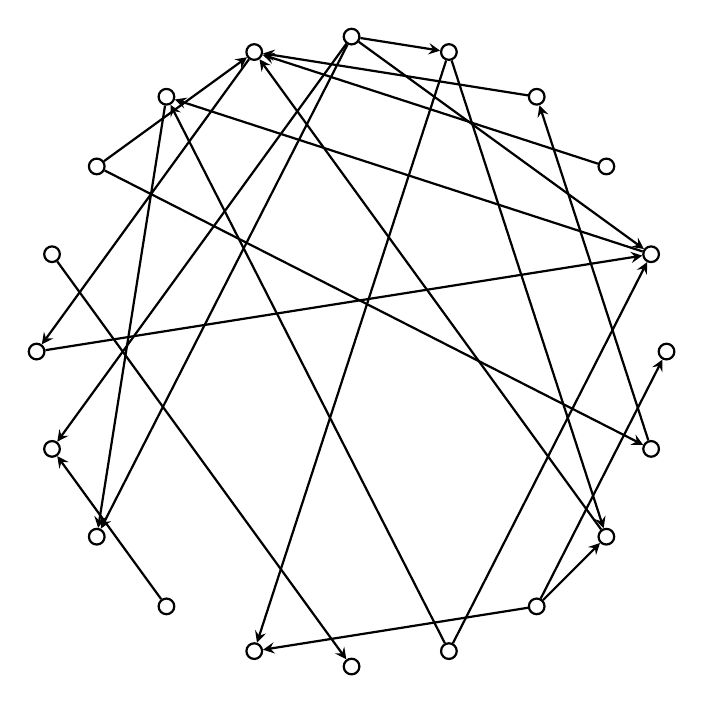
\begin{tikzpicture}
[lineDecorate/.style={->,>=stealth,thick},%
  nodeDecorate/.style={shape=circle,inner sep=2pt,draw,thick},
  scale=4]
%% nodes or vertices
\foreach \nodename/\x/\y in {
  0/1.00000000000000/0.000000000000000,
  1/0.951056516295154/0.309016994374947,
  2/0.809016994374947/0.587785252292473,
  3/0.587785252292473/0.809016994374947,
  4/0.309016994374947/0.951056516295154,
  5/0.000000000000000/1.00000000000000,
  6/-0.309016994374947/0.951056516295154,
  7/-0.587785252292473/0.809016994374947,
  8/-0.809016994374947/0.587785252292473,
  9/-0.951056516295154/0.309016994374947,
  10/-1.00000000000000/0.000000000000000,
  11/-0.951056516295154/-0.309016994374947,
  12/-0.809016994374947/-0.587785252292473,
  13/-0.587785252292473/-0.809016994374947,
  14/-0.309016994374947/-0.951056516295154,
  15/0.000000000000000/-1.00000000000000,
  16/0.309016994374947/-0.951056516295154,
  17/0.587785252292473/-0.809016994374947,
  18/0.809016994374947/-0.587785252292473,
  19/0.951056516295154/-0.309016994374947}
{
  \node (\nodename) at (\x,\y) [nodeDecorate] {};
}
%% edges or lines
\path
\foreach \startnode/\endnode in {
  1/7, 2/6, 3/6, 4/14, 4/18, 5/1, 5/4, 5/11, 5/12, 6/10, 7/12, 8/6,
  8/19, 9/15, 10/1, 13/11, 16/1, 16/7, 17/0, 17/14, 17/18, 18/6, 19/3}
{
  (\startnode) edge[lineDecorate] node {} (\endnode)
};
\end{tikzpicture}
\end{figure}

\end{document}

\caption{A random oriented graph generated using a graph in
  $G(20,\, 0.1)$ and cutoff probability $0.5$.}
\label{fig:random_graphs:random_oriented_graph}
\end{figure}

%% One of the first properties of random graphs which makes them so pleasant to work with is the following

%% \begin{theorem}
%%   Let $H$ be any graph, and $0<p<1$. Then
%% $$\lim_{n\to +\infty}P\left[H\text{ is an induced subgraph of }G_{n,p}\right]=1$$
%% \end{theorem}
%% \begin{proof}[Sketch]
%% Instinctively, we would like to find a copy of $H$ in $G_{n,p}$ by iteratively finding an acceptable representant $h(v_i)$ in $G_{n,p}$ of every vertex $v_i$ of $V(H) = \{v_1, \dots, v_k\}$. How could such a strategy work ?
%% \begin{itemize}
%% \item Pick for $v_1$ any vertex $h(v_1)\in G_{n,p}$
%% \item Pick for $v_2$ any vertex $h(v_2)\in G_{n,p}$ such that $h(v_1)h(v_2)\in E(G_{n,p})$ if $v_1v_2\in E(H)$, and such that $h(v_1)h(v_2)\not \in E(G_{n,p})$ otherwise
%% \item \dots
%% \item Assuming you have found, for all $i\leq j\leq k$, a representant $h(v_i)$ for each vertex $v_i$, and such that $H[\{v_1,\dots,v_{j-1}\}]$ is isomorphic to $G_{n,p}[\{h(v_1),\dots,h(v_{j-1})\}]$, try to find a new vertex $h(v_j)$ such that $\forall i<j,h(v_i)h(v_j)\in E(G_{n,p})$ if  and only if $v_iv_j\in E(H)$.

%%   When $n$ is growing large, such a vertex will exist with high probability.
%% \end{itemize}
%% \end{proof}

%% \begin{proof}
%%   Formally, let us write $H_i = H[\{v_1,\dots,v_{j-1}\}]$, and denote
%%   the probability that $H$ is an induced subgraph of $G_{n,p}$ by $P[H
%%     \mapsto_{ind} G_{n,p}]$. We can roughly bound the probability that $H_i$, but not $H_{i+1}$, is an induced subgraph of $G_{n,p}$ the following way :

%%   \begin{itemize}
%%   \item We put a copy of $H_i$ at any of the $\binom n i$ different $i$-subsets of $V(G_{n,p})$.

%%     This can be done, each time, in $i!$ different ways as the vertices $\{v_1, \dots, v_i\}$ can be permuted

%%   \item We compute the probability that no other vertex of $G_{n,p}$ can be used to complete our current copy of $H_i$ into a copy of $H_{i+1}$. The probability that such a vertex is acceptable being
%%     $$p^{d_{H_{i+1}}(v_{i+1})}(1-p)^{i-d_{H_{i+1}}(v_{i+1})}\geq min(p, 1-p)^i$$
%%     the property that none of the $n-i$ vertices left is acceptable is at most
%%     $$\left({ 1- min(p, 1-p)^i } \right)^{(n-i)}$$
%%   \end{itemize}

%%   As $0<p<1$, we can write $0<\epsilon = min(p, 1-p)$ and thus, the probability that $H_i$, but not $H_{i+1}$, is a induced subgraph of $G_{n,p}$ is at most $$i!\binom n i (1-\epsilon^i)^{n-i}\leq i! n^i (1-\epsilon^i)^{n-i} = o(1/n)$$
%% Which is asymptotically equal to 0 as $n$ grows.

%% Thus

%% \begin{align*}
%%   P[H \mapsto_{ind} G_{n,p}]&=1 - P[H_2 \mapsto_{ind} G_{n,p}, H_3\not \mapsto_{ind} G_{n,p}]\\
%%   &-P[H_3 \mapsto_{ind} G_{n,p}, H_4\not \mapsto_{ind} G_{n,p}]\\
%%   &\dots\\
%%   &-P[H_{k-1} \mapsto_{ind} G_{n,p}, H_k\not \mapsto_{ind} G_{n,p}]\\
%%   P[H \mapsto_{ind} G_{n,p}]&\geq 1-\sum_{i\leq k}i!n^i(1-\epsilon^i)^{n-i}\\
%%   &\geq 1-k\times o(1/n)\\
%% \end{align*}

%% Which proves the result.

%% \end{proof}

%% This proof also gives us a simple algorithm to find a copy of a graph $H$ into a random graph $G_{n,p}$. While obviously such an algorithm will not always find the copy of $H$ if it exists, the probability of a successful run will tend toward $1$ as proved immediately above.

%% \begin{lstlisting}
%% def find_induced(H, G):

%%     # f is the function from V(H) to V(G) we
%%     # are attempting to define
%%     f = {}

%%     # leftovers is the set of vertices of G which have not yet
%%     # been used by f
%%     G_leftovers = G.vertices()

%%     # Set of vertices for which no representant has been found yet
%%     H_leftovers = H.vertices()

%%     # While the function is not complete
%%     while H_leftovers:

%%         # We look for the next vertex of H
%%         v = H_leftovers.pop(0)

%%         # ... and look for its possible image
%%         candidates = [u for u in G_leftovers if
%%           all([ H.has_edge(h,v) == G.has_edge(f_h,u)
%%             for h,f_h in f.iteritems()])]

%%         if not candidates:
%%             raise ValueError("No copy of H has been found in G")

%%         # We pick the first of them
%%         f[v] = candidates[0]
%%         G_leftovers.remove(f[v])

%%     return f
%% \end{lstlisting}


%%%%%%%%%%%%%%%%%%%%%%%%%%%%%%%%%%%%%%%%%%%%%%%%%%%%%%%%%%%%%%%%%%%%%%%%%%%

\section{Small-world networks}
\label{sec:random_graphs:small_world_networks}

%% The small-world network model of Watts and
%% Strogatz~\cite{WattsStrogatz1998}. The economic small-world model of
%% Latora and Marchiori~\cite{LatoraMarchiori2003}. See also
%% Milgram~\cite{Milgram1967}, Newman~\cite{Newman2003b}, and Albert and
%% Barab{\'a}si~\cite{AlbertBarabasi2002}. Adapt Figure 1 from page
%% 432 of Travers and Milgram~\cite{TraversMilgram1969} resulting
%% Milgram's small-world experiment. See Barrat and
%% Weigt~\cite{BarratWeigt2000} for some properties of small-world
%% networks.

Many real-world networks exhibit the
\emph{small-world effect}\index{small-world!effect}: that most pairs
of distinct vertices in the network are connected by relatively short
path lengths. The small-world effect was empirically
demonstrated~\cite{Milgram1967} in a famous~1960s experiment by
Stanley Milgram\index{Milgram, Stanley}, who distributed a number
of letters to a random selection of people. Recipients were instructed
to deliver the letters to the addressees on the condition that letters
must be passed to people whom the recipients knew on a first-name
basis. Milgram found that on average six steps were required for a
letter to reach its target recipient, a number now immortalized in the
phrase\index{six degrees of separation} ``six degrees of
separation''~\cite{Guare1990}. The small-world effect has been studied
and verified for many real-world networks including
%%
\begin{itemize}
\item social\index{network!social}: collaboration network of actors in
  feature films~\cite{AmaralEtAl2000,WattsStrogatz1998}, scientific
  publication
  authorship~\cite{CastroGrossman1999,GrossmanIon1995,Newman2001a,Newman2001b};

\item information\index{network!information}: citation
  network~\cite{Redner1998}, Roget's\index{Roget's Thesaurus}
  Thesaurus~\cite{Knuth1993}, word
  co-occurrence~\cite{DorogovtsevMendes2001,FerrerSole2001};

\item technological\index{network!technological}:
  internet~\cite{ChenEtAl2002,FaloutsosEtAl1999}, power
  grid~\cite{WattsStrogatz1998}, train routes~\cite{SenEtAl2003},
  software~\cite{Newman2003a,ValverdeEtAl2002};

\item biological\index{network!biological}: metabolic
  network~\cite{JeongEtAl2000}, protein
  interactions~\cite{JeongEtAl2001}, food
  web~\cite{HuxhamEtAl1996,Martinez1991}, neural
  network~\cite{WattsStrogatz1998,WhiteEtAl1986}.
\end{itemize}

Watts\index{Watts, Duncan J.} and\index{Strogatz, Steven H.}
Strogatz~\cite{Watts1999a,Watts1999b,WattsStrogatz1998}
proposed a network model that exhibits the small-world effect. Let $n$
and $k$ be positive integers such that $n \gg k \gg \ln n \gg 1$~(in
particular, $0 < k < n/2$), $k$ being even, and consider a probability
$0 < p < 1$. Starting from an undirected
$k$-circulant\index{regular graph!$k$-circulant} graph $G = (V,E)$ on
$n$ vertices, the Watts-Strogatz\index{Watts-Strogatz model} model
proceeds to rewire each edge with probability $p$. The rewiring
procedure works as follows. Let $V$ be uniformly distributed. For each
$v \in V$, let $e \in E$ be an edge having $v$ as an endpoint. Choose
another $u \in V$ different from $v$. With probability $p$, delete the
edge $e$ and add the edge $vu$. The rewiring must produce a
simple\index{simple graph} graph with the same order and size as
$G$. As $p \to 1$, the graph $G$ goes from $k$-circulant to exhibiting
properties of $\cG(n,p)$\index{random graph!binomial}. Small-world
networks are intermediate between $k$-circulant and binomial random
graphs. The Watts-Strogatz model is said to provide a procedure for
interpolating between the latter two types of graphs.

The last paragraph contains an algorithm for rewiring edges of a
graph. While the algorithm is simple, in practice it potentially skips
over a number of vertices to be considered for rewiring. If
$G = (V,E)$ is a $k$-circulant graph on $n$ vertices and $p$ is the
rewiring probability, the candidate vertices to be rewired follow a
geometric distribution with parameter $p$. This geometric trick,
essentially the same speed-up technique used by the Batagelj-Brandes
Algorithm~\ref{alg:random_graphs:linear_generate_random_sparse_Gnp},
can be used to speed up the rewiring algorithm. To elaborate, suppose
$G$ has vertex set $V = \{0, 1, \dots, n-1\}$. If $r$ is chosen
uniformly at random from the interval $(0,1)$, the index of the vertex
to be rewired can be obtained from
\[
1 + \left\lfloor \frac{\ln(1 - r)} {\ln(1 - p)} \right\rfloor.
\]
The above geometric method is incorporated into
Algorithm~\ref{alg:random_graphs:generate_Watts_Strogatz_graph} to
generate a Watts-Strogatz network in worst-case runtime
$O(nk + m)$, where $n$ and $k$ are as per the input of the algorithm
and $m$ is the size of the $k$-circulant graph on $n$ vertices. Note
that lines~\ref{alg:Watts_Strogatz:even_index}
to~\ref{alg:Watts_Strogatz:choose_vertex_odd_index} are where we avoid
self-loops and multiple edges.

\begin{algorithm}[!htbp]
\index{algorithm!random}
\index{complete graph}
\index{list!contiguous edge}
\index{regular graph!$k$-circulant}
\index{small-world!algorithm}
\index{small-world!network}
\index{Watts-Strogatz model}
%%%%%%%%%%%%%%%%%%%%%%%%%%%%%%%%%%%%%%%%%%%%%%%%%%%%%%%%%%%%%%%%%%%%%%%%%%%
%% This file is part of the book
%%
%% Algorithmic Graph Theory
%% http://code.google.com/p/graph-theory-algorithms-book/
%%
%% Copyright (C) 2009, 2010, 2011 Minh Van Nguyen <nguyenminh2@gmail.com>
%%
%% See the file COPYING for copying conditions.
%%%%%%%%%%%%%%%%%%%%%%%%%%%%%%%%%%%%%%%%%%%%%%%%%%%%%%%%%%%%%%%%%%%%%%%%%%%

\DontPrintSemicolon
\SetAlgoNoLine
%%
%% data section
\SetKwInOut{Input}{Input}
\SetKwInOut{Output}{Output}
%%
%% input/output
\Input{Positive integer $n$ denoting the number of vertices. Positive
  even integer $k$ for the degree of each vertex, where
  $n \gg k \gg \ln n \gg 1$. In particular, $k$ should satisfy
  $0 < k < n/2$. Rewiring probability $0 < p \leq 1$.}
\Output{A Watts-Strogatz network on $n$ vertices.}
\BlankLine
%%
%% algorithm body
$M \assign nk$~\tcc*[f]{sum of all vertex degrees = twice number of edges}\;
$r \assign$ draw uniformly at random from $[0,1)$\;
$v \assign 1 + \lfloor \log(1 - r) / \log(1 - p) \rfloor$\;
$E \assign$ contiguous edge list of $k$-circulant graph on $n$ vertices\;
\While{$v \leq M$}{
  $u \assign$ draw uniformly at random from $[0, 1, \dots, n-1]$\;
  $E[v-1] \assign u$\;
  $r \assign$ draw uniformly at random from $[0,1)$\;
  $v \assign v + 1 + \lfloor \log(1 - r) / \log(1 - p) \rfloor$\;
}
$G \assign \overline{K_n}$\;
$\ell \assign |E|$\;
add edge $v_i v_{i+1}$ to $G$ for even $0 \leq i \leq \ell - 2$\;
\Return $G$\;

\caption{Watts-Strogatz network model.}
\label{alg:random_graphs:generate_Watts_Strogatz_graph}
\end{algorithm}


%%%%%%%%%%%%%%%%%%%%%%%%%%%%%%%%%%%%%%%%%%%%%%%%%%%%%%%%%%%%%%%%%%%%%%%%%%%

\subsubsection{Characteristic path length}

Watts and Strogatz~\cite{WattsStrogatz1998} analyzed the structure of
networks generated by
Algorithm~\ref{alg:random_graphs:generate_Watts_Strogatz_graph} via
two quantities: the
\emph{characteristic path length}\index{small-world!characteristic path length}
$\ell$ and the
\emph{clustering coefficient}\index{small-world!clustering coefficient}
$C$. Let $G = (V,E)$ be a Watts-Strogatz network as generated by
Algorithm~\ref{alg:random_graphs:generate_Watts_Strogatz_graph}, where
the vertex set is $V = \{0, 1, \dots, n-1\}$. For each pair of
vertices $i,j \in V$, let $d_{ij}$ be the distance from $i$ to $j$. If
there is no path from $i$ to $j$ or $i = j$, set $d_{ij} = 0$. Thus
\[
d_{ij}
=
\begin{cases}
0, & \text{if there is no path from $i$ to $j$}, \\[4pt]
0, & \text{if $i = j$}, \\[4pt]
k, & \text{where $k$ is the length of a shortest path from $i$ to $j$}.
\end{cases}
\]
Since $G$ is undirected, we have $d_{ij} = d_{ji}$. Consequently when
computing the distance between each distinct pair of vertices, we
should avoid double counting by computing $d_{ij}$ for $i < j$. Then
the characteristic path length of $G$ is defined by
%%
\begin{equation}
\label{eqn:random_graphs:define_characteristic_path_length}
\begin{aligned}
\ell(G)
&=
\frac{1}{n(n-1)/2} \cdot \frac{1}{2} \sum_{i \neq j} d_{ij} \\[4pt]
&=
\frac{1}{n(n-1)} \sum_{i \neq j} d_{ij}
\end{aligned}
\end{equation}
%%
which is averaged over all possible pairs of distinct vertices,
i.e. the number of edges in the complete\index{complete graph} graph
$K_n$.

It is inefficient to compute the characteristic path length via
equation~\eqref{eqn:random_graphs:define_characteristic_path_length}
because we would effectively sum $n(n - 1)$ distance values. As $G$ is
undirected, note that
\[
\frac{1}{2} \sum_{i \neq j} d_{ij}
=
\sum_{i < j} d_{ij}
=
\sum_{i > j} d_{ij}.
\]
The latter equation holds for the following reason. Let $D = [d_{ij}]$
be a matrix of distances for $G$, where $i$ is the row index, $j$ is
the column index, and $d_{ij}$ is the distance from $i$ to $j$. The
required sum of distances can be obtained by summing all entries
above~(or below) the main diagonal of $D$. Therefore the
characteristic path length can be expressed as
%%
\begin{align*}
\ell(G)
&=
\frac{2}{n(n-1)} \sum_{i < j} d_{ij} \\[4pt]
&=
\frac{2}{n(n-1)} \sum_{i > j} d_{ij}
\end{align*}
%%
which requires summing $\frac{n(n-1)}{2}$ distance values.


%%%%%%%%%%%%%%%%%%%%%%%%%%%%%%%%%%%%%%%%%%%%%%%%%%%%%%%%%%%%%%%%%%%%%%%%%%%

\subsubsection{Clustering coefficient}

The \emph{clustering coefficient}\index{small-world!clustering coefficient} of a
simple graph $G$ quantifies the ``cliquishness'' of vertices in
$G = (V,E)$. This quantity is thus said to be a local property of
$G$. Watts and Strogatz~\cite{WattsStrogatz1998} defined the
clustering coefficient as follows. Suppose $n = |V| > 0$ and let $n_i$
count the number of neighbors of vertex $i \in V$, a quantity that is
equivalent to the degree of $i$, i.e. $\deg(i) = n_i$. The complete
graph $K_{n_i}$ on the $n_i$ neighbors of $i$ has $n_i(n_i - 1) / 2$
edges. The \emph{neighbor graph}\index{neighbor graph} $\cN_i$ of $i$
is a subgraph of $G$, consisting of all vertices~($\neq i$) that are
adjacent to $i$ and preserving the adjacency relation among those
vertices as found in the supergraph $G$. For example, given the graph
in Figure~\ref{fig:neighbor_graph:original_graph} the neighbor graph
of vertex $10$ is shown in
Figure~\ref{fig:neighbor_graph:neighbor_graph}. The local clustering
coefficient $C_i$ of $i$ is the ratio
\[
C_i
=
\frac{N_i} {n_i (n_i - 1) / 2}
\]
where $N_i$ counts the number of edges in $\cN_i$. In case $i$ has
degree $\deg(i) < 2$, we set the local clustering coefficient of $i$
to be zero. Then the clustering
coefficient\index{small-world!clustering coefficient} of $G$ is defined by
\[
C(G)
=
\frac{1}{n} \sum_{i \in V} C_i
=
\frac{1}{n} \sum_{i \in V} \frac{N_i} {n_i (n_i - 1) / 2}.
\]

\begin{figure}[!htbp]
\centering
\index{neighbor graph}
%%%%%%%%%%%%%%%%%%%%%%%%%%%%%%%%%%%%%%%%%%%%%%%%%%%%%%%%%%%%%%%%%%%%%%%%%%%
%% This file is part of the book
%%
%% Algorithmic Graph Theory
%% http://code.google.com/p/graph-theory-algorithms-book/
%%
%% Copyright (C) 2009--2011 Minh Van Nguyen <nguyenminh2@gmail.com>
%%
%% See the file COPYING for copying conditions.
%%%%%%%%%%%%%%%%%%%%%%%%%%%%%%%%%%%%%%%%%%%%%%%%%%%%%%%%%%%%%%%%%%%%%%%%%%%

\documentclass{article}

\usepackage{subfigure}
\usepackage{tikz}
\usetikzlibrary{external}
\tikzexternalize{neighbor-graph}
\newcommand{\cN}{\mathcal{N}}

\begin{document}

\begin{figure}
\subfigure[Graph on $11$ vertices.]{
\label{fig:neighbor_graph:original_graph}
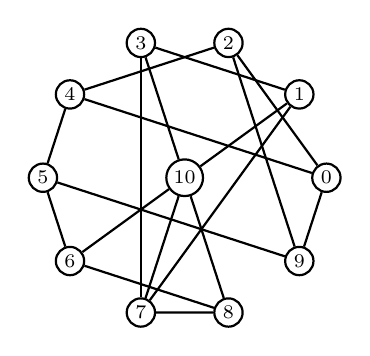
\begin{tikzpicture}
[lineDecorate/.style={-,thick},%
  nodeDecorate/.style={shape=circle,inner sep=1.5pt,draw,thick},
  scale=1.8]
\scriptsize
%% nodes or vertices
\foreach \nodename/\x/\y in {
  0/1.00000000000000/0.000000000000000,
  1/0.809016994374947/0.587785252292473,
  2/0.309016994374947/0.951056516295154,
  3/-0.309016994374947/0.951056516295154,
  4/-0.809016994374947/0.587785252292473,
  5/-1.00000000000000/0.000000000000000,
  6/-0.809016994374947/-0.587785252292473,
  7/-0.309016994374947/-0.951056516295154,
  8/0.309016994374947/-0.951056516295154,
  9/0.809016994374947/-0.587785252292473,
  10/0/0}
{
  \node (\nodename) at (\x,\y) [nodeDecorate] {$\nodename$};
}
%% edges or lines
\path
\foreach \startnode/\endnode in {
  0/2, 0/4, 0/9, 1/3, 1/7, 2/4, 2/9, 3/7, 4/5, 5/6, 5/9, 6/8, 7/8,
  10/1, 10/3, 10/6, 10/7, 10/8}
{
  (\startnode) edge[lineDecorate] node {} (\endnode)
};
\end{tikzpicture}
}
%%
%%
\qquad
\subfigure[$\cN_{10}$]{
\label{fig:neighbor_graph:neighbor_graph}
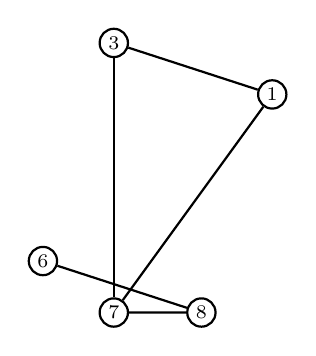
\begin{tikzpicture}
[lineDecorate/.style={-,thick},%
  nodeDecorate/.style={shape=circle,inner sep=1.5pt,draw,thick},
  scale=1.8]
\scriptsize
%% nodes or vertices
\foreach \nodename/\x/\y in {
  1/0.809016994374947/0.587785252292473,
  3/-0.309016994374947/0.951056516295154,
  6/-0.809016994374947/-0.587785252292473,
  7/-0.309016994374947/-0.951056516295154,
  8/0.309016994374947/-0.951056516295154}
{
  \node (\nodename) at (\x,\y) [nodeDecorate] {$\nodename$};
}
%% edges or lines
\path
\foreach \startnode/\endnode in {1/3, 1/7, 3/7, 6/8, 7/8}
{
  (\startnode) edge[lineDecorate] node {} (\endnode)
};
\end{tikzpicture}
}
\end{figure}

\end{document}

\caption{The neighbor graph of a vertex.}
\label{fig:random_graphs:neighbor_graph}
\end{figure}

Consider the case where we have a $k$-circulant graph
$G = (V,E)$ on $n$ vertices and a rewiring probability $p = 0$. That
is, we do not rewire any edge of $G$. Each vertex of $G$ has degree
$k$. Let  $k' = k/2$. Then the $k$ neighbors of each vertex in $G$ has
$3k' (k' - 1) / 2$ edges between them, i.e. each neighbor graph
$\cN_i$ has size $3k' (k' - 1) / 2$. Then the clustering coefficient
of $G$ is
\[
\frac{3(k' - 1)} {2(2k' - 1)}.
\]
When the rewiring probability is $p > 0$, Barrat and
Weigt~\cite{BarratWeigt2000} showed that the clustering coefficient of
any graph $G'$ in the Watts-Strogatz network model~(see
Algorithm~\ref{alg:random_graphs:generate_Watts_Strogatz_graph}) can
be approximated by
\[
C(G')
\approx
\frac{3(k' - 1)} {2(2k' - 1)} (1 - p)^3.
\]


%%%%%%%%%%%%%%%%%%%%%%%%%%%%%%%%%%%%%%%%%%%%%%%%%%%%%%%%%%%%%%%%%%%%%%%%%%%

\section{Scale-free networks}

The power-law degree distribution model of Barab{\'a}si and
Albert~\cite{BarabasiAlbert1999}. See also Newman~\cite{Newman2003b},
and Albert and Barab{\'a}si~\cite{AlbertBarabasi2002}.


%%%%%%%%%%%%%%%%%%%%%%%%%%%%%%%%%%%%%%%%%%%%%%%%%%%%%%%%%%%%%%%%%%%%%%%%%%%

\section{Evolving networks}

Preferential attachment models. See Newman~\cite{Newman2003b},
and Albert and Barab{\'a}si~\cite{AlbertBarabasi2002}. Adapt figures
from~\cite{HeartEtAl1978} on the growth of ARPANET.


%%%%%%%%%%%%%%%%%%%%%%%%%%%%%%%%%%%%%%%%%%%%%%%%%%%%%%%%%%%%%%%%%%%%%%%%%%%

\section{Problems}

\begin{problem}
\item Modify Algorithm~\ref{alg:random_graphs:random_simple_graph} to
  generate the following random graphs.
  %%
  \begin{enumerate}[(a)]
  \item Simple weighted, undirected graph.

  \item Simple digraph.

  \item Simple weighted digraph.
  \end{enumerate}

\begin{algorithm}[!htbp]
\index{algorithm!random}
\index{complete graph}
\index{simple graph!random}
%%%%%%%%%%%%%%%%%%%%%%%%%%%%%%%%%%%%%%%%%%%%%%%%%%%%%%%%%%%%%%%%%%%%%%%%%%%
%% This file is part of the book
%%
%% Algorithmic Graph Theory
%% http://code.google.com/p/graph-theory-algorithms-book/
%%
%% Copyright (C) 2009, 2010, 2011 Minh Van Nguyen <nguyenminh2@gmail.com>
%%
%% See the file COPYING for copying conditions.
%%%%%%%%%%%%%%%%%%%%%%%%%%%%%%%%%%%%%%%%%%%%%%%%%%%%%%%%%%%%%%%%%%%%%%%%%%%

\DontPrintSemicolon
\SetAlgoNoLine
%%
%% data section
\SetKwInOut{Input}{Input}
\SetKwInOut{Output}{Output}
%%
%% input/output
\Input{Positive integer $n$ and a probability $0 < p < 1$.}
\Output{A random graph from $G(n,p)$.}
\BlankLine
%%
%% algorithm body
$G \assign \overline{K_n}$\;
$V \assign \{1, 2, \dots, n\}$\;
\For{$i \assign 1, 2, \dots, n - 1$}{
  \For{$j \assign i + 1, i + 2, \dots, n$}{
    $r \assign$ draw uniformly at random from $[0,1)$\;
    \If{$r < p$}{
      add edge $ij$ to $G$\;
    }
  }
}
\Return $G$\;

\caption{Quadratic generation of a random graph in $\cG(n,p)$.}
\label{alg:random_graphs:quadratic_generate_random_Gnp}
\end{algorithm}

\begin{algorithm}[!htbp]
\index{algorithm!random}
\index{complete graph}
\index{simple graph!random}
%%%%%%%%%%%%%%%%%%%%%%%%%%%%%%%%%%%%%%%%%%%%%%%%%%%%%%%%%%%%%%%%%%%%%%%%%%%
%% This file is part of the book
%%
%% Algorithmic Graph Theory
%% http://code.google.com/p/graph-theory-algorithms-book/
%%
%% Copyright (C) 2009--2011 Minh Van Nguyen <nguyenminh2@gmail.com>
%%
%% See the file COPYING for copying conditions.
%%%%%%%%%%%%%%%%%%%%%%%%%%%%%%%%%%%%%%%%%%%%%%%%%%%%%%%%%%%%%%%%%%%%%%%%%%%

\DontPrintSemicolon
\SetAlgoNoLine
%%
%% data section
\SetKwData{MyMax}{max}
\SetKwData{MyTrue}{True}
%%
%% input
\KwIn{Positive integers $n$ and $N$ such that $1 \leq N \leq \binom{n}{2}$.}
%%
%% output
\KwOut{A random graph from $G(n,N)$.}
\BlankLine
%%
%% algorithm body
$\MyMax \assign \binom{n}{2}$\;
\If{\rm $n = 1$ or $N = \MyMax$}{
  \Return $K_n$\;
}
$G \assign \overline{K_n}$\;
$u \assign 0$\;
$v \assign 1$\;
$t \assign 0$\tcc*[f]{number of candidates processed so far}\;
$k \assign 0$\tcc*[f]{number of edges selected so far}\;
\While{$\MyTrue$}{
  $r \assign$ draw uniformly at random from $\{0, 1, \dots, \MyMax - t\}$\;
  \If{$r < N - k$}{
    add edge $uv$ to $G$\;
    $k \assign k + 1$\;
    \If{$k = N$}{
      \Return $G$\;
    }
  }
  $t \assign t + 1$\;
  $v \assign v + 1$\;
  \If{$v = n$}{
    $u \assign u + 1$\;
    $v \assign u + 1$\;
  }
}

\caption{Briggs' algorithm for random graph in $\cG(n,N)$.}
\label{alg:random_graphs:Briggs_random_GnN}
\end{algorithm}

\item\label{prob:random_graphs:quadratic_generate_random_Gnp}
  Algorithm~\ref{alg:random_graphs:generate_random_Gnp} can be
  considered as a template for generating random graphs in
  $\cG(n,p)$. The procedure does not specify how to generate all the
  $2$-combinations of a set of $n > 1$ objects. Here we discuss how to
  construct all such $2$-combinations and derive a quadratic time
  algorithm for generating random graphs in $\cG(n,p)$.
  %%
  \begin{enumerate}[(a)]
  \item Consider a vertex set $V = \{0, 1, \dots, n - 1\}$ with at
    least two elements and let $E$ be the set of all $2$-combinations
    of $V$, where each $2$-combination is written $ij$. Show that
    $ij \in E$ if and only if $i < j$.

  \item From the previous exercise, we know that if $0 \leq i < n - 1$
    then there are $n - (i + 1)$ pairs $jk$ where either $i = j$ or
    $i = k$. Show that
    \[
    \sum_{i=0}^{n-2} (n - i - 1)
    =
    \frac{n^2 - n}{2}
    \]
    and conclude that
    Algorithm~\ref{alg:random_graphs:quadratic_generate_random_Gnp}
    has worst-case runtime $O((n^2 - n) / 2)$.
  \end{enumerate}

\item Modify the Batagelj-Brandes
  Algorithm~\ref{alg:random_graphs:linear_generate_random_sparse_Gnp}
  to generate the following types of graphs.
  %%
  \begin{enumerate}[(a)]
  \item Directed simple graphs.

  \item Directed acyclic graphs.

  \item Bipartite graphs.
  \end{enumerate}

\item Repeat the previous problem for
  Algorithm~\ref{alg:random_graphs:expected_linear_generate_random_GnN}.

\item In~2006, Keith M. Briggs\index{Briggs!Keith M.}
  provided~\cite{Briggs2011} an algorithm that generates a random
  graph in $\cG(n,N)$, inspired by Knuth's\index{Knuth!Algorithm~S}
  Algorithm~S~(Selection sampling technique) as found on page~142 of
  Knuth\index{Knuth!Donald E.}~\cite{Knuth1998b}. Pseudocode of
  Briggs' algorithm is presented in
  Algorithm~\ref{alg:random_graphs:Briggs_random_GnN}.
  %%
  \begin{enumerate}[(a)]
  \item Provide runtime analysis of
    Algorithm~\ref{alg:random_graphs:Briggs_random_GnN} and compare
    your results with those presented in
    section~\ref{sec:random_graphs:Erdos_Renyi_model}.

  \item Under which conditions would Briggs' algorithm be more
    efficient than
    Algorithm~\ref{alg:random_graphs:expected_linear_generate_random_GnN}?
  \end{enumerate}

\item Briggs'\index{Briggs!algorithm}
  Algorithm~\ref{alg:random_graphs:Briggs_random_GnN} follows the
  general template of an algorithm that samples without replacement
  $n$ items from a pool of $N$ candidates. Here $0 < n \leq N$ and the
  size $N$ of the candidate pool is known in advance. However there
  are situations where the value of $N$ is not known beforehand, and
  we wish to sample without replacement $n$ items from the candidate
  pool. What we know is that the candidate pool has enough members to
  allow us to select $n$ items. Vitter's\index{Vitter!Jeffrey Scott}
  algorithm~R~\cite{Vitter1985}, called
  reservoir\index{reservoir sampling} sampling, is suitable for the
  situation and runs in $O(n (1 + \ln(N/n)))$ expected time.
  %%
  \begin{enumerate}[(a)]
  \item Describe and provide pseudocode of
    Vitter's\index{Vitter!algorithm} algorithm.

  \item Prove the correctness of Vitter's algorithm.

  \item Provide runtime analysis of Vitter's algorithm.
  \end{enumerate}

\item Repeat Example~\ref{eg:random_graphs:random_oriented_graph} but
  using each of Algorithms~\ref{alg:random_graphs:generate_random_Gnp}
  and~\ref{alg:random_graphs:expected_linear_generate_random_GnN}.

\item Diego Garlaschelli\index{Garlaschelli, Diego}
  introduced~\cite{Garlaschelli2009} in~2009 a weighted version of the
  $\cG(n,p)$ model, called the weighted\index{random graph!weighted}
  random graph model. Denote by $\cG_W(n,p)$ the weighted random graph
  model.
  %%
  \begin{enumerate}[(a)]
  \item Provide a description and pseudocode of a procedure to
    generate a graph in $\cG_W(n,p)$.

  \item Analyze the runtime complexity of the algorithm.

  \item Describe various statistical physics properties of $\cG_W(n,p)$.
  \end{enumerate}
\end{problem}
